\documentclass[tikz,border=10pt]{standalone}
\usepackage{ctex} % 若需中文支持
\usetikzlibrary{arrows.meta, calc}

\begin{document}

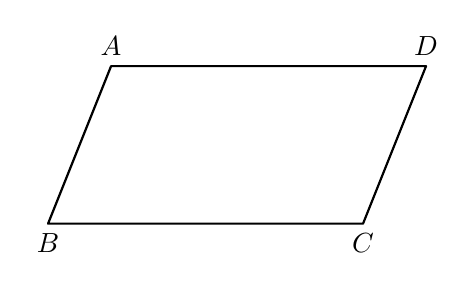
\begin{tikzpicture}[line cap=round, line join=round, >=Stealth, thick]
    % --- 参数定义 ---
    % 定义平行四边形的宽度 w，高度 h，以及底角的偏移量 offset
    \def\w{4}
    \def\h{2}
    \def\offset{0.8}

    % --- 坐标点定义 ---
    % 按照逆时针或题目习惯定位四个顶点
    \coordinate (B) at (0, 0);           % 左下角
    \coordinate (C) at (\w, 0);          % 右下角
    \coordinate (D) at (\w+\offset, \h); % 右上角
    \coordinate (A) at (\offset, \h);    % 左上角

    % --- 绘制图形边界 ---
    \draw (A) -- (B) -- (C) -- (D) -- cycle;

    % --- 标注顶点名称 ---
    % 这里的 italic 字体符合数学绘图规范，通过 label 自动定位
    \node [above] at (A) {$A$};
    \node [below] at (B) {$B$};
    \node [below] at (C) {$C$};
    \node [above] at (D) {$D$};

\end{tikzpicture}

\end{document}